\chapter{Relations and Sequences}

\section{Relations}
\begin{definition}[Binary Relations]
    A binary relation $R$ from a set $A$ to a set $B$ is a subset of the Cartesian product $A \times B$. In other words, $R$ is a set of ordered pairs $(a, b)$ where $a \in A$ and $b \in B$. We write $a R b$ to indicate that the pair $(a, b)$ is in the relation $R$.
\end{definition}

\begin{eg}
    Let $A = \{0,1\}$ and $B = \{a,b,c\}$, then:
    \begin{itemize}[itemsep=1pt,label=$\circ$]
        \item $A \times B = \{(0,a), (0,b), (0,c), (1,a), (1,b), (1,c)\}$
        \item $R_1 = \{(0,a), (1,b)\}$ is a relation from $A$ to $B$
        \item $R_2 = \{(0,b), (1,c)\}$ is another relation from $A$ to $B$
    \end{itemize}
\end{eg}
A binary relation $R$ on a set $A$ itself is a subset of $A \times A$. In this case, we say that $R$ is a relation on $A$.
\begin{eg}
    Let $A = \{0,1\}$, then:
    \begin{itemize}[itemsep=1pt,label=$\circ$]
        \item $A \times A = \{(0,0), (0,1), (1,0), (1,1)\}$
        \item $R_1 = \{(0,0), (1,1)\}$ is a relation on $A$
        \item $R_2 = \{(0,1), (1,0)\}$ is another relation on $A$
    \end{itemize}
\end{eg}
On a set $A$, there can be many relations. In fact:
\begin{itemize}[itemsep=1pt,label=$\circ$]
    \item $A \times A$ has $|A|^2$ elements when $A$ has $|A|$ elements.
    \item Every subset of $A \times A$ can be a relation.
    \item Therefore, there are $2^{|A|^2}$ possible relations on a set $A$.
\end{itemize}

\subsection{Properties of Relations}
\begin{definition}[Reflexive Relation]
    A relation $R$ on a set $A$ is called reflexive if for every element $a \in A$, the pair $(a, a)$ is in the relation $R$. In other words, every element is related to itself.
\end{definition}
Note that the empty relation on a empty set is reflexive.
\begin{eg}
    Let $A = \{0,1\}$, then:
    \begin{itemize}[itemsep=1pt,label=$\circ$]
        \item $R_1 = \{(0,0), (1,1)\}$ is reflexive
        \item $R_2 = \{(0,1), (1,0)\}$ is not reflexive
        \item $R_3 = \{(0,0), (0,1), (1,0), (1,1)\}$ is reflexive
    \end{itemize}
\end{eg}

\begin{definition}[Symmetric Relation]
    A relation $R$ on a set $A$ is called symetric if for every pair $(a, b) \in R$, the pair $(b, a)$ is also in $R$. In other words, if $a$ is related to $b$, then $b$ is also related to $a$.
\end{definition}
\begin{eg}
    Let $A = \{0,1\}$, then:
    \begin{itemize}[itemsep=1pt,label=$\circ$]
        \item $R_1 = \{(0,0), (1,1)\}$ is symetric
        \item $R_2 = \{(0,1), (1,0)\}$ is symetric
        \item $R_3 = \{(0,0), (0,1), (1,0), (1,1)\}$ is symetric
        \item $R_4 = \{(0,0), (0,1)\}$ is not symetric
    \end{itemize}
\end{eg}

\begin{definition}[Antisymmetric Relation]
    A relation $R$ on a set $A$ is called antisymmetric if and only if $(a,b) \in R$ and $(b,a) \in R$ then $a = b, \ \forall a,b \in A$.
\end{definition}
\begin{eg}
    Let $A = \{0,1\}$, then:
    \begin{itemize}[itemsep=1pt,label=$\circ$]
        \item $R_1 = \{(0,0), (1,1)\}$ is antisymmetric
        \item $R_2 = \{(0,1), (1,0)\}$ is not antisymmetric
        \item $R_3 = \{(0,0), (0,1), (1,0), (1,1)\}$ is not antisymmetric
        \item $R_4 = \{(0,0), (0,1)\}$ is antisymmetric
    \end{itemize}
\end{eg}

\begin{definition}[Transitive Relation]
    A relation $R$ on a set $A$ is called transitive if for every pair $(a, b) \in R$ and $(b, c) \in R$, the pair $(a, c)$ is also in $R$. In other words, if $a$ is related to $b$ and $b$ is related to $c$, then $a$ is also related to $c$.
\end{definition}
\begin{eg}
    Let $A = \{0,1,2\}$, then:
    \begin{itemize}[itemsep=1pt,label=$\circ$]
        \item $R_1 = \{(0,0), (1,1), (2,2)\}$ is transitive
        \item $R_2 = \{(0,1), (1,0)\}$ is not transitive
        \item $R_3 = \{(0,0), (0,1), (1,0), (1,1)\}$ is not transitive
        \item $R_4 = \{(0,0), (0,1), (1,1), (1,2), (0,2)\}$ is transitive
        \item $R_5 = \{(0,0), (0,1), (1,1), (1,2)\}$ is not transitive
    \end{itemize}
\end{eg}

\subsection{Combining Relations}
\begin{definition}[Combining Relations]
    Given two relations $R_1$ and $R_2$ on a set $A$, we can combine them using basic operations to form new ones such as:
    \begin{itemize}[itemsep=1pt,label=$\circ$]
        \item Union: $R_1 \cup R_2 = \{(a,b) \ | \ (a,b) \in R_1 \text{ or } (a,b) \in R_2\}$
        \item Intersection: $R_1 \cap R_2 = \{(a,b) \ | \ (a,b) \in R_1 \text{ and } (a,b) \in R_2\}$
        \item Subtraction: $R_1 - R_2 = \{(a,b) \ | \ (a,b) \in R_1 \text{ and } (a,b) \notin R_2\}$
        \item Composition: $R_1 \circ R_2 = \{(a,c) \ | \ \exists b \in A, (a,b) \in R_1 \text{ and } (b,c) \in R_2\}$
    \end{itemize}
\end{definition}
\begin{eg}
    Let $A = \{0,1\}$, $R_1 = \{(0,0), (1,1)\}$ and $R_2 = \{(0,1), (1,0)\}$, then:
    \begin{itemize}[itemsep=1pt,label=$\circ$]
        \item $R_1 \cup R_2 = \{(0,0), (1,1), (0,1), (1,0)\}$
        \item $R_1 \cap R_2 = \emptyset$
        \item $R_1 - R_2 = R_1$
        \item $R_2 - R_1 = R_2$
        \item $R_1 \circ R_2 = \{(0,1), (1,0)\} = R_2$
        \item $R_2 \circ R_1 = \{(0,1), (1,0)\} = R_2$
    \end{itemize}
\end{eg}

\subsection{Equivalence Relations and Classes}
\begin{definition}[Equivalence Relation]
    A relation $R$ on a set $A$ is called an equivalence relation if it is reflexive, symmetric, and transitive.
\end{definition}
Two elements $a$ and $b$ that are related by an equivalence relation are called equivalent. The notation $a \sim b$ is often used to denote that $a$ is equivalent to $b$.
\begin{eg}
    Let $A = \{a,b,c\}$, the relation $R = \{(a,a), (b,b), (c,c), (a,b), (b,a)\}$ is an equivalence relation because:
    \begin{itemize}[itemsep=1pt,label=$\circ$]
        \item Reflexive: $(a,a), (b,b), (c,c) \in R$
        \item Symmetric: $(a,b) \in R \Rightarrow (b,a) \in R$
        \item Transitive: There are no pairs $(a,b)$ and $(b,c)$ in $R$ such that $(a,c)$ is not in $R$
    \end{itemize}
\end{eg}

\begin{eg}
    Let $R = \{(a,b) \in \mathbb{R} \times \mathbb{R} \mid a -b \in \mathbb{Z}\}$ be an equivalence relation, then:
    \begin{itemize}[itemsep=1pt,label=$\circ$]
        \item Reflexive: $a - a = 0$, $0 \in \mathbb{Z}$
        \item Symmetric: $a - b \in \mathbb{Z}$, then $b - a \in \mathbb{Z}$
        \item Transitive: $a - b \in \mathbb{Z}$ and $b - c \in \mathbb{Z}$, then $(a -b) + (b-c) = a - c \in \mathbb{Z}$
    \end{itemize}
\end{eg}

\begin{definition}[Equivalence Class]
    Given an equivalence relation $R$ on a set $A$ and an element $a \in A$, the equivalence class of $a$, denoted by $[a]$, is the set of all elements in $A$ that are equivalent to $a$ under the relation $R$. In other words:
    \[ [a] = \{b \in A \ | \ a R b\} \]
\end{definition}
\begin{eg}
    Let $A = \{a,b,c\}$ and $R = \{(a,a), (b,b), (c,c), (a,b), (b,a)\}$ be an equivalence relation on $A$, then:
    \begin{itemize}[itemsep=1pt,label=$\circ$]
        \item The equivalence class of $a$ is $[a] = \{a,b\}$
        \item The equivalence class of $b$ is $[b] = \{a,b\}$
        \item The equivalence class of $c$ is $[c] = \{c\}$
    \end{itemize}
\end{eg}

\begin{theorem}
    Let $R$ be an equivalence relation on a set $A$. Then the three following statements for element $a$ and $b$ of $A$ are equivalent:
    \begin{itemize}[itemsep=1pt,label=$\circ$]
        \item $(a,b) \in R$
        \item $[a]_R = [b]_R$
        \item $[a]_R \cap [b]_R \neq \emptyset$
    \end{itemize}
\end{theorem}
\begin{proof}
    Let's prove that these statements are equivalent by showing that (1) implies (2), (2) implies (3), and (3) implies (1). \\
    \textbf{(1) implies (2):} Assume that $(a,b) \in R$. We need to show that $[a]_R = [b]_R$. \\
    Let $c \in [a]_R \subseteq A$. We have:
    \[
        (a, c) \in R \quad \text{and} \quad (a,b) \in R
    \]
    Since $R$ is symmetric we have that $(b,a) \in R$ and thus by transitivity we have:
    \[
        (a,c) \in R \quad \text{and} \quad (b,a) \in R \implies (b,c) \in R
    \]
    Therefore, $c \in [b]_R$. This shows that $[a]_R \subseteq [b]_R$. By a similar argument, we can show that $[b]_R \subseteq [a]_R$. Hence, $[a]_R = [b]_R$. \\
    \textbf{(2) implies (3):} Assume that $[a]_R = [b]_R$. We need to show that $[a]_R \cap [b]_R \neq \emptyset$. \\
    Since $R$ is reflexive, we have $(a,a) \in R$, which implies that $[a]_R$ contains at least $a$. Therefore, $[a]_R \cap [b]_R$ contains at least $a$, and hence it is not empty. \\
    \textbf{(3) implies (1):} Assume that $[a]_R \cap [b]_R \neq \emptyset$. We need to show that $(a,b) \in R$. \\
    Since $\exists c \in [a]_R \land c \in [b]_R$, we have:
    \[
        (a,c) \in R \quad \text{and} \quad (b,c) \in R
    \]
    Since $R$ is symmetric, we have $(c,b) \in R$. By transitivity, we have:
    \[
        (a,c) \in R \quad \text{and} \quad (c,b) \in R \implies (a,b) \in R
    \]
    This completes the proof that the three statements are equivalent.
\end{proof}

\subsection{Partitions}
\begin{definition}[Partition]
    A partition of a set $A$ is a collection of non-empty, disjoint subsets of $A$ whose union is $A$. It can be formally defined as follows:
    \begin{itemize}[itemsep=1pt,label=$\circ$]
        \item Each subset in the partition is non-empty: $\forall S_i \in P, S_i \neq \emptyset$
        \item The subsets are pairwise disjoint: $\forall S_i, S_j \in P, i \neq j \implies S_i \cap S_j = \emptyset$
        \item The union of all subsets in the partition is the entire set $A$: $\bigcup_{S_i \in P} S_i = A$
    \end{itemize}
\end{definition}
Every equivalence relation on a set $A$ induces a partition of $A$ into equivalence classes. Conversely, every partition of a set $A$ defines an equivalence relation on $A$.
\begin{eg}
    Let $A = \{1, 2, 3, \ldots\}$ and $R = \{(a, b) \mid a - b \text{ is divisible by } 5\} = \{(a, b) \mid a - b = 5k \text{ for some } k \in \mathbb{Z}\}$ be an equivalence relation on $A$. Then the equivalence classes are:
    \begin{itemize}[itemsep=1pt,label=$\circ$]
        \item $[0]_R = \{0, 5, 10, 15, \ldots\}$
        \item $[1]_R = \{1, 6, 11, 16, \ldots\}$
        \item $[2]_R = \{2, 7, 12, 17, \ldots\}$
        \item $[3]_R = \{3, 8, 13, 18, \ldots\}$
        \item $[4]_R = \{4, 9, 14, 19, \ldots\}$
        \item $[5]_R = \{5, 10, 15, 20, \ldots\} \subset [0]_R$
    \end{itemize}
    The partition of $A$ induced by the equivalence relation $R$ is:
    \[ P = \{[1], [2], [3], [4], [0]\} \]
\end{eg}

\subsection{Partial and Total Orders}
\begin{definition}[Partial Order]
    A relation $R$ on a set $A$ is called a partial order if it is reflexive, antisymmetric, and transitive. A set $A$ equipped with a partial order $R$ is called a partially ordered set or poset, denoted by $(A, R)$.
\end{definition}

\begin{eg}
    Let $R = \{(a,b) \in \mathbb{Z} \times \mathbb{Z} \mid a \geq b\}$. We want to show that $R$ is a partial order on $\mathbb{Z}$.
    \begin{itemize}[itemsep=1pt,label=$\circ$]
        \item Reflexive: For any integer $a$, $a \geq a$
        \item Antisymmetric: If $a \geq b$ and $b \geq a$, then $a = b$
        \item Transitive: If $a \geq b$ and $b \geq c$, then $a \geq c$
    \end{itemize}
    Therefore, $R$ is a partial order on $\mathbb{Z}$ and $(\mathbb{Z}, \geq)$ is a poset.
\end{eg}
Note that the symbol $\preceq$ is used to denote the partial ordering relation in an arbitrary poset.

\begin{eg}
    Let's take the divide relation on $\mathbb{Z}^+$. We show that it is a partial order.
    \begin{itemize}[itemsep=1pt,label=$\circ$]
        \item Reflexive: For any positive integer $a$, $a \mid a$
        \item Antisymmetric: If $a \mid b$ and $b \mid a$, then $a = b$
        \item Transitive: If $a \mid b$ and $b \mid c$, then $a \mid c$
    \end{itemize}
    Therefore, the divide relation is a partial order on $\mathbb{Z}^+$ and $(\mathbb{Z}^+, \mid)$ is a poset.
\end{eg}

\begin{definition}[Comparable Elements]
    In a poset $(A, R)$, two elements $a$ and $b$ in $A$ are said to be comparable if either $a R b$ or $b R a$. If neither $a R b$ nor $b R a$, then $a$ and $b$ are said to be incomparable.
\end{definition}
Note that its not necessary that every pair of elements in a poset are comparable.

\begin{eg}
    Consider the poset $(\mathbb{Z}^+, \mid)$. The elements $2$ and $3$ are incomparable because neither $2 \mid 3$ nor $3 \mid 2$. However, the elements $2$ and $4$ are comparable because $2 \mid 4$.
\end{eg}

\begin{definition}[Total Order]
    A relation $R$ on a set $A$ is called a total order (or linear order) if it is a partial order and every pair of elements in $A$ are comparable. A set $A$ equipped with a total order $R$ is called a totally ordered set or chain, denoted by $(A, R)$.
\end{definition}

\begin{eg}
    The poset $(\mathbb{Z}, \leq)$ is a total order because:
    \begin{itemize}[itemsep=1pt,label=$\circ$]
        \item Reflexive: For any integer $a$, $a \leq a$
        \item Antisymmetric: If $a \leq b$ and $b \leq a$, then $a = b$
        \item Transitive: If $a \leq b$ and $b \leq c$, then $a \leq c$
        \item Comparable: For any integers $a$ and $b$, either $a \leq b$ or $b \leq a$
    \end{itemize}
    Therefore, $(\mathbb{Z}, \leq)$ is a totally ordered set but $(\mathbb{Z}^+, \mid)$ is not.
\end{eg}

\begin{definition}[Well-Order]
    A total order $R$ on a set $A$ is called a well-order if every non-empty subset of $A$ has a least element with respect to the order $R$. In other words, for any non-empty subset $S \subseteq A$, there exists an element $m \in S$ such that for all elements $s \in S$, $m R s$.
\end{definition}

\begin{eg}
    Let's check for the following posets if they are ordered or well-ordered:
    \begin{itemize}[itemsep=1pt,label=$\circ$]
        \item $(\mathbb{Z}, \geq)$ is a total order but not a well-order because the subset of negative integers does not have a least element.
        \item $(\mathbb{Z}^+, \mid)$ is a partial order but not a total order because not every pair of positive integers are comparable.
        \item $(\mathbb{Z}^+, \leq)$ is a well-order because every non-empty subset of positive integers has a least element.
    \end{itemize}
\end{eg}

\subsection{Hasse Diagrams}
\begin{definition}[Hasse Diagram]
    A Hasse diagram is a graphical representation of a finite partially ordered set (poset). It is a way to visualize the elements of the poset and the order relations between them. In a Hasse diagram:
    \begin{itemize}[itemsep=1pt,label=$\circ$]
        \item Each element of the poset is represented by a vertex (or node).
        \item An edge (or line) is drawn between two vertices $a$ and $b$ if $a R b$ and there is no element $c$ such that $a R c$ and $c R b$ (i.e., $b$ covers $a$).
        \item The edges are drawn such that if $a R b$, then vertex $b$ is placed higher than vertex $a$ in the diagram.
        \item Reflexive and transitive relations are not explicitly shown in the diagram.
    \end{itemize}
\end{definition}
\begin{eg}
    Let's consider the poset $(\{1,2,3,4\}, \leq)$. The Hasse diagram for this poset is:
    \begin{center}
        \begin{tikzpicture}[scale=1]
            \node[] (1) at (0,0) {1};
            \node (2) at (0,1) {2};
            \node (3) at (0,2) {3};
            \node (4) at (0,3) {4};
            \draw (1) -- (2);
            \draw (2) -- (3);
            \draw (3) -- (4);
        \end{tikzpicture}
    \end{center}
\end{eg}

\begin{eg}
    Let's draw the Hasse diagram of $(\mathcal{P}(\{x,y\}), \subseteq)$ with $\mathcal{P}(\{x,y\}) = \{\emptyset, \{x\}, \{y\}, \{x,y\}\}$. The Hasse diagram is:
    \begin{center}
        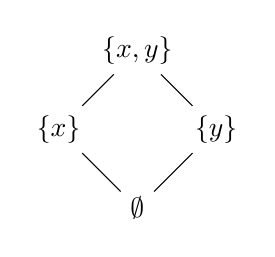
\begin{tikzpicture}[scale=1]
            \node[] (empty) at (0,0) {$\emptyset$};
            \node (x) at (-1,1) {$\{x\}$};
            \node (y) at (1,1) {$\{y\}$};
            \node (xy) at (0,2) {$\{x,y\}$};
            \draw (empty) -- (x);
            \draw (empty) -- (y);
            \draw (x) -- (xy);
            \draw (y) -- (xy);
        \end{tikzpicture}
    \end{center}
\end{eg}

\begin{definition}[Lexicographic Order]
    Given two posets $(A, R_A)$ and $(B, R_B)$, the lexicographic order on the Cartesian product $A \times B$ is defined as follows: For any two pairs $(a_1, b_1), (a_2, b_2) \in A \times B$, we say that $(a_1, b_1) \preceq (a_2, b_2)$ if either:
    \begin{itemize}[itemsep=1pt,label=$\circ$]
        \item $a_1 R_A a_2$, or
        \item $a_1 = a_2$ and $b_1 R_B b_2$
    \end{itemize}
\end{definition}
\begin{eg}
    Let's consider the posets $(\mathbb{Z}^+, \leq)$ and $(\mathbb{Z}^+, \leq)$ then $(\mathbb{Z}^+ \times \mathbb{Z}^+, \prec)$ is a poset with the lexicographic order represented by:
    \begin{center}
        \begin{tikzpicture}
            \foreach \i in {1,2,...,7} {
                \foreach \j in {1,2,...,7} {
                    \ifnumless{\i}{3}{
                        \node[circle, draw, fill=primary, primary, inner sep=1pt] (\i\j) at (\i*1.2,\j) {};
                        \node[primary] at (\i*1.2,\j) [below=2pt] {(\i,\j)};
                    }{
                        \ifnumequal{\i}{3}{
                            \ifnumless{\j}{4}{
                                \node[circle, draw, fill=primary, primary, inner sep=1pt] (\i\j) at (\i*1.2,\j) {};
                                \node[primary] at (\i*1.2,\j) [below=2pt] {(\i,\j)};
                            }{
                                \node[circle, draw, fill, inner sep=1pt] (\i\j) at (\i*1.2,\j) {};
                                \node[] at (\i*1.2,\j) [below=2pt] {(\i,\j)};
                            }
                        }{
                            \node[circle, draw, fill, inner sep=1pt] (\i\j) at (\i*1.2,\j) {};
                            \node at (\i*1.2,\j) [below=2pt] {(\i,\j)};
                        }
                    }
                    \ifnumequal{\j}{7}{
                        \node at (\i*1.2,\j) [above=5pt] {$\vdots$};
                    }{}
                    \ifnumequal{\i}{7}{
                        \node at (\i*1.2,\j) [right=5pt] {$\ldots$};
                }{}
                }
            }
        \end{tikzpicture}
    \end{center}
    Where all of the colored nodes are the elements that are less than $(3,4)$.
\end{eg}

\section{Sequences}
\begin{definition}[Sequence]
    A sequence is an ordered list of elements of a set, which can be finite or infinite. A sequence can be defined as a function from the set of natural numbers (or a subset of natural numbers) to a set of elements.
\end{definition}
\begin{eg}
    Some examples of sequences are:
    \begin{itemize}[itemsep=1pt,label=$\circ$]
        \item $1,2,3,4,5,8$
        \item $c,o,m,p,u,t,e,r$
        \item $1,3,9,27,81, \ldots$
        \item $1,1,1,1,1,\ldots$
    \end{itemize}
\end{eg}

\subsection{Arithmetic and Geometric Progressions}
\begin{definition}[Arithmetic Progression]
    An arithmetic progression (or arithmetic sequence) is a sequence of numbers in which the difference between any two consecutive terms is constant. This constant difference is called the common difference, denoted by $d$. If the first term of the sequence is $a_1$, then the $n$-th term of the arithmetic progression can be expressed as:
    \[ a_n = a_1 + (n-1)d \]
    The sum of the first $n$ terms of an arithmetic progression, denoted by $S_n$, can be calculated using the formula:
    \[ S_n = \frac{n}{2} (2a_1 + (n-1)d) \]
    or equivalently:
    \[ S_n = \frac{n}{2} (a_1 + a_n) \]
\end{definition}

\begin{definition}[Geometric Progression]
    A geometric progression (or geometric sequence) is a sequence of numbers in which the ratio between any two consecutive terms is constant. This constant ratio is called the common ratio, denoted by $r$. If the first term of the sequence is $a_1$, then the $n$-th term of the geometric progression can be expressed as:
    \[ a_n = a_1 \cdot r^{n-1} \]
    The sum of the first $n$ terms of a geometric progression, denoted by $S_n$, can be calculated using the formula:
    \[ S_n = a_1 \frac{1 - r^n}{1 - r} \quad \text{if } r \neq 1 \]
    If $|r| < 1$ and the sequence is infinite, the sum to infinity can be calculated as:
    \[ S = \frac{a_1}{1 - r} \]
\end{definition}

\begin{eg}
    Some example of arithmetic and geometric progressions are:
    \begin{itemize}[itemsep=1pt,label=$\circ$]
        \item $1,4,9,16,25,\ldots$ (not an arithmetic or geometric progression)
        \item $1,\frac{1}{2},\frac{1}{4},\frac{1}{8},\ldots$ (Geometric Progression)
        \item $7,4,1,-2,-5,\ldots$ (Arithmetic Progression)
        \item $1,2,6,24,120,720$ (not an arithmetic or geometric progression)
    \end{itemize}
\end{eg}

\subsection{Strings}
\begin{definition}[Strings]
    A string is a finite sequence of characters from a given alphabet. An alphabet is a finite set of symbols or characters. It can be more formally defined as:
    \[
        f: \{0,1,\ldots, n\} \to A
    \]
    The empty string, denoted by $\lambda$, is the string with zero length.
\end{definition}

\begin{eg}
    Let's consider the lowercase English alphabet then the ordering used in dictionaries is a lexicographic order on the set of all strings that can be formed from this alphabet. For example:
    \begin{itemize}[itemsep=1pt,label=$\circ$]
        \item "apple" comes before "banana" because 'a' comes before 'b'
        \item "discreet" comes before "discrete" because 'e' comes before 't'
        \item "cat" comes before "catalog" because "cat" is a prefix of "catalog"
    \end{itemize}
    Strings with lexicographic ordering are well-ordered sets.
\end{eg}